%	The main skeletal structure
	\documentclass[crop,tikz,convert={outext=.svg,command=\unexpanded{pdf2svg \infile\space\outfile}},multi=false]{standalone}%	\documentclass[twocolumn]{report}
	\usepackage{setspace}
	\usepackage{graphicx}
		\DeclareGraphicsExtensions{.pdf,.png,.eps,.svg	ps}
	\usepackage{subcaption}
	\usepackage{lscape}
	\usepackage{pifont}
%	\usepackage{bbding}
	\usepackage{multirow}
	\usepackage{longtable}
	\usepackage[version=4]{mhchem}
	\usepackage{xfrac}
	\usepackage{color}
	\usepackage[colorlinks=true]{hyperref}
	\usepackage{gensymb}
	\usepackage{multicol}
		\setlength{\columnseprule}{0.4pt}
		\setlength{\columnsep}{5mm}
\makeatletter 
\newcounter{reaction} 
%%% >> for article << 
%\renewcommand\thereaction{C\,\arabic{reaction}} 
%%% << for article << 
%%% >> for report and book >> 
\renewcommand\thereaction{C\,\thechapter.\arabic{reaction}} 
\@addtoreset{reaction}{chapter} 
%%% << for report and book << 
\newcommand\reactiontag{\refstepcounter{reaction}\tag{\thereaction}} 
\newcommand\reaction@[2][]{\begin{equation}\ce{#2}% 
\ifx\@empty#1\@empty\else\label{#1}\fi% 
\reactiontag\end{equation}} 
\newcommand\reaction@nonumber[1]{\begin{equation*}\ce{#1}% 
\end{equation*}} 
\newcommand\reaction{\@ifstar{\reaction@nonumber}{\reaction@}} 
\makeatother 


	\usepackage[a4paper]{geometry}
	\usepackage{fullpage}
	\usepackage{fancyhdr}
%		\pagestyle{fancy}
%		\lhead{}
%		\chead{}
%		\rhead{\slshape \rightmark}
%		\fancyhead[LO,RE]{\slshape \leftmark} 
%		\fancyfoot[R]{\thepage} 
%	\renewcommand{\headrulewidth}{0.4pt} 
%	\renewcommand{\footrulewidth}{0.4pt} 
	\usepackage{cite}
	
%	\onehalfspacing
	\renewcommand{\baselinestretch}{1.5}
	
%	Footnote symbols
	\renewcommand{\thefootnote}{\fnsymbol{footnote}}

% Defining the chapter abstract area
%	\newenvironment{abstract}{\rightskip1in}{}

% Allow standard state notation
	\usepackage[varioref=false]{chemstyle}

% Allow for numbered examples
%	\usepackage{theorem,lipsum}
%	\theorembodyfont{\upshape}
%	\newtheorem{example}{Example}[chapter]
%	\newtheorem{question}{Question}[chapter]
%	\newtheorem{exercise}{Exercise}[chapter]
%	\newtheorem{concept}{Key Concept}[chapter]
%%%%%\begin{example}
%%%%%This is an example?
%%%%%\end{example}
%%%%%
%%%%%\begin{question}
%%%%%This is a quesiton?
%%%%%\end{question}

%%%%%FONT STUFF

%\usepackage[defaultfam,extralight,tabular,lining]{montserrat} %% Option 'defaultfam'
%%% only if the base font of the document is to be sans serif
%\usepackage[T1]{fontenc}
%\renewcommand*\oldstylenums[1]{{\fontfamily{Montserrat-TOsF}\selectfont #1}}

\usepackage{arev}
\usepackage[T1]{fontenc}
\usepackage{soul}

%%%%%TIKZ stuff
	\usepackage{tikz}
	\usepackage{pgfplots}
	\usetikzlibrary{decorations.pathmorphing,patterns,arrows,shapes.arrows,shapes}
	\usepgfplotslibrary{fillbetween}
	\tikzset{every picture/.style=remember picture}
		\newcommand{\mathnode}[1]{%
		\mathord{\tikz[baseline=(#1.base), inner sep = 0pt]{\node (#1) {$#1$};}}}

%%%%%% Grey stuff
%Need to define a shitload of greys...
\definecolor{gray1}{RGB}{240,240,240}
\definecolor{gray2}{RGB}{225,225,225}
\definecolor{gray3}{RGB}{210,210,210}
\definecolor{gray4}{RGB}{200,200,200}
\definecolor{gray5}{RGB}{180,180,180}


\begin{document}


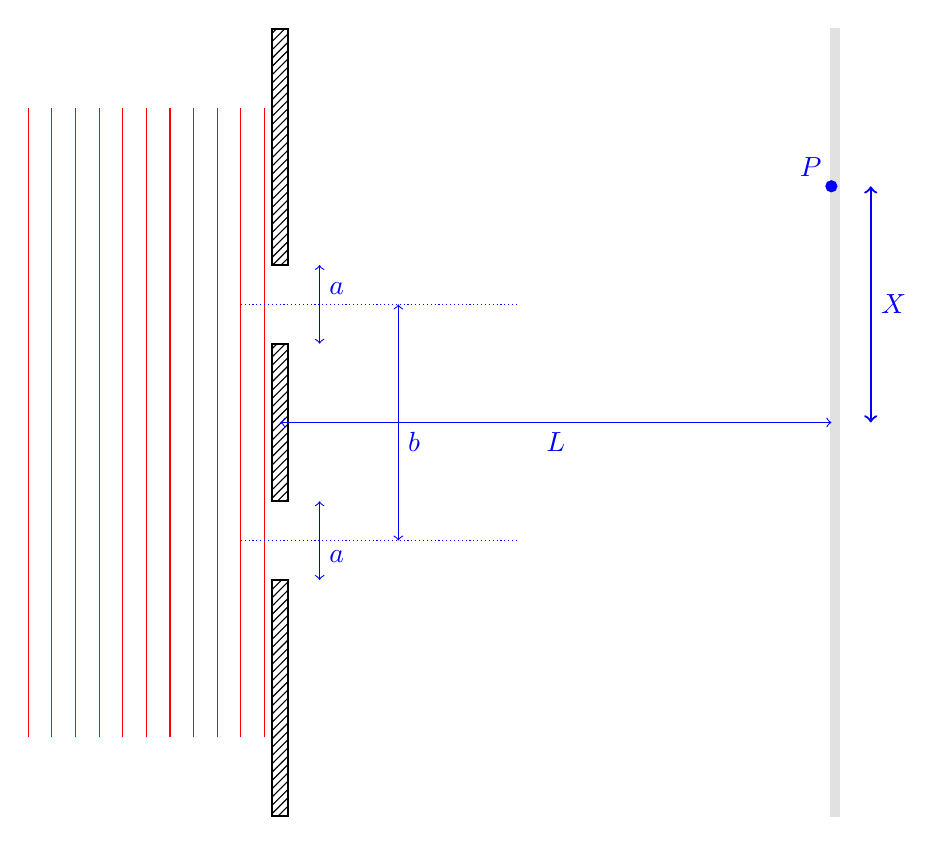
\begin{tikzpicture}[scale=1]
%  \begin{axis}[
%    grid=none,
%    axis lines = middle,
%    xmax=2,
%    ymax=2, 
%    ymin = -2,
%    xmin = -2,
%%    axis x line=none,   
%%   width=10cm,
%%    height=5cm, 
%%    axis y line=none,
%%    restrict y to domain=-1:9,
%    enlargelimits,
%%    xlabel={$x$},
%%    xlabel style={ },
%%    ylabel={$y$},
%%    ylabel style={},
%    ticks=none,
%%    ylabel near ticks,
%%    xlabel near ticks,
%    ]
%% Incident wave:
	\newcommand \heightofwall{5}
	\newcommand \slitsep{3}
	\newcommand \slitwidth{1}
	\newcommand \wallwidth{0.2}
	\newcommand \waveheight{4}
	\newcommand \wavespace{0.3}
	\newcommand \waveoffset{0.2}
	\newcommand \distancetoscreen{7}
	\newcommand \screenheight{5}
	\newcommand \pointP{3}
	\newcommand \subfigX{4}
	\newcommand \subfigY{-4}
	\newcommand \subfigrad{3.5}
	\filldraw [draw=black, thick, pattern = north east lines] (-{0.5*\wallwidth},{(\slitsep+\slitwidth)/2}) rectangle ({0.5*\wallwidth},{\heightofwall});
	\filldraw [draw=black, thick, pattern = north east lines] (-{0.5*\wallwidth},-{(\slitsep-\slitwidth)/2}) rectangle ({0.5*\wallwidth},{(\slitsep-\slitwidth)/2});
	\filldraw [draw=black, thick, pattern = north east lines] (-{0.5*\wallwidth},-{(\slitsep+\slitwidth)/2}) rectangle ({0.5*\wallwidth},-{\heightofwall});
	
	
\foreach \a in {0,...,10}
{
\draw[red](-{(\waveoffset+\a*\wavespace)},-\waveheight) -- (-{(\waveoffset+\a*\wavespace)},+\waveheight);
}	

	\draw[blue,densely dotted] (-0.5,{\slitsep/2}) -- (3,{\slitsep/2});
	\draw[blue,densely dotted] (-0.5,-{\slitsep/2}) -- (3,-{\slitsep/2});
	\draw[blue,<->] (1.5,-{\slitsep/2}) -- node[below right]{$b$} (1.5,{\slitsep/2});
	\draw[blue,<->] (0.5,-{(\slitsep-\slitwidth)/2}) -- node[below right]{$a$} (0.5,-{(\slitsep+\slitwidth)/2});
	\draw[blue,<->] (0.5,{(\slitsep-\slitwidth)/2}) -- node[above right]{$a$} (0.5,{(\slitsep+\slitwidth)/2});

\filldraw [draw=black, thick, gray2]({\distancetoscreen},{-\screenheight}) rectangle ({\distancetoscreen+0.5*\wallwidth},{\screenheight});
\draw[blue,<->] (0,0) -- node[below]{$L$} ({\distancetoscreen},0);
\filldraw[blue] ({\distancetoscreen},{\pointP}) circle(2pt) node[above left]{$P$};
%\draw[red](0,{\slitsep/2}) -- ({\distancetoscreen},{\pointP});
%\draw[red](0,-{\slitsep/2}) -- ({\distancetoscreen},{\pointP});
\draw[blue,<->,thick] ({\distancetoscreen+0.5},0) -- node[right]{$X$} ({\distancetoscreen+0.5},\pointP);
%\draw[<->] (0:0.8*\distancetoscreen) arc  (0:11.8:0.8*\distancetoscreen) node[midway,right]{ $\theta$} ;
%\draw[<->,red] (2,{\slitsep/2}) arc  (0:10:2) node[midway,right]{ $\theta_1$} ;
%\draw[<->,red] (2,-{\slitsep/2}) arc  (0:12:2) node[midway,right]{ $\theta_2$} ;


%\draw[black,thick](0,0) circle (1);
%
%\draw[black,densely dotted, thick](55:1) -- ++ (-20:4);
%\draw[black,densely dotted, thick](-135:1) -- ++ (-72:4);

%% Subfigure

%\draw[black,thick](\subfigX,\subfigY) circle (\subfigrad);
%	\filldraw [draw=black, thick, pattern = north east lines] ({0.7*\subfigX-0.5*\wallwidth},{3*(\slitsep+\slitwidth)/2 + \subfigY}) rectangle ({0.7*\subfigX+0.5*\wallwidth},{3*(\slitsep+\slitwidth) + \subfigY-0.7});
%	\filldraw [draw=black, thick, pattern = north east lines] ({0.7*\subfigX-0.5*\wallwidth},{\subfigY-3*(1.2*\slitsep-\slitwidth)/2}) rectangle ({0.7*\subfigX+0.5*\wallwidth},{3*(1.2*\slitsep-\slitwidth)/2 +\subfigY});
%	\filldraw [draw=black, thick, pattern = north east lines] ({0.7*\subfigX-0.5*\wallwidth},{\subfigY-3*(\slitsep+\slitwidth)/2}) rectangle ({0.7*\subfigX+0.5*\wallwidth},{\subfigY+0.7-3*(\slitsep+\slitwidth)});
%	
%	\draw[blue,densely dotted] ({-0.5+0.7*\subfigX},{\subfigY+3.3*\slitsep/2}) node[ left]{$S_1$}-- ({3+0.7*\subfigX},{\subfigY+3.3*\slitsep/2});
%	\draw[blue,densely dotted] ({-0.5+0.7*\subfigX},{\subfigY-3.3*\slitsep/2}) node[ left]{$S_2$} -- ({3+0.7*\subfigX},{\subfigY-3.3*\slitsep/2});
%	\draw[blue,<->] ({-0.3+0.7*\subfigX},{\subfigY+3.3*\slitsep/2}) -- node[left]{$d$} ({-0.3+0.7*\subfigX},{\subfigY-3.3*\slitsep/2});
%	\draw[red,thick] ({0.7*\subfigX},{\subfigY+3.3*\slitsep/2}) -- ++ (11:3.8);
%	\draw[red,thick] ({0.7*\subfigX},{\subfigY-3.3*\slitsep/2}) -- ++ (11:4.7);
%	\draw[blue,thick,densely dotted] ({0.7*\subfigX},{\subfigY+3.3*\slitsep/2})  -- ++ (-79:4.5);
%	\draw[blue,thick,densely dotted] ({0.7*\subfigX},{\subfigY-3.3*\slitsep/2}) -- ++ (-79:1.5);
%	\draw[<->,red] (2+\subfigX,{\subfigY-3.3*\slitsep/2}) arc  (0:18:2) node[midway,right]{ $\theta$} ;
%	\draw[<->,red] (0.7*\subfigX,{\subfigY-2.5*\slitsep/2}) arc  (-90:-70:1.5) node[right]{ $\theta$} ;
%	\draw[<->,blue,thick] (0.7*\subfigX+0.2,{\subfigY-5*\slitsep/2}) -- ++ (11:0.6) node[right]{$d\sin \theta$};


%	\draw[->, thick,black] (axis cs:{(\deltaX+90)/180},1) -- ++ (axis direction cs:0.5,0) node[above]{$v$};
	
%	\draw[->,thick,red] (axis cs:0,{sin(-\deltaX)}) -- ++({atan(2*cos(-\deltaX))}:1cm) node[right]{$F$};
%	\draw[densely dotted,red] (axis cs:0,{sin(-\deltaX)}) -- ++(0:0.5cm) node[above]{\footnotesize $\theta$};
	
%	\draw[->,ultra thick,cyan] (axis cs:0,{sin(-\deltaX)}) -- ++(axis direction cs:0,{-0.5*cos(\deltaX)}) node[right]{\footnotesize $f$};
%	\node[draw,circle,fill=red,inner sep=0pt, minimum size=3pt] at  (axis cs:0,{sin(-\deltaX)}) {};
%	\node[] at (axis cs:-0.15,1) {$y$};
%	\node[] at (axis cs:4,-0.15) {$x$};

%    \addplot[blue,domain=0:3.7,samples=100,] {sin(180*x-\deltaX)}; % Incident pulse
 
%\end{axis}

\end{tikzpicture}
\end{document}

% Use the following to include the graphics in the chapter
%
%
%\begin{figure}[htbp]
%\begin{center}
%\includegraphics[scale=1]{ch-x/images/filename.pdf}
%\caption[Caption for list of figures]{Full caption to appear beside the image}
%\label{fig:label}
%\end{center}
%\end{figure}
 